% Geometry, font
\documentclass[12pt, letter]{article}
\usepackage[margin=0.8in]{geometry}
\usepackage[T1]{fontenc}
\usepackage{fourier}
\usepackage{titling}
\setlength{\droptitle}{-5em} 
\usepackage[parfill]{parskip}
\usepackage{graphicx}
\graphicspath{{imgs/}}
\usepackage{hyperref}

% Math stuff
\usepackage{amssymb}
\usepackage{amsmath}
\usepackage{bm}

% Code Highlighting
\usepackage{minted}
\usemintedstyle{solarizedlight}

\author{Zach Neveu}
\title{ Day 22 Notes }

\begin{document}
\maketitle

\section{Agenda}%
\label{sec:agenda}

\begin{itemize}
	\item Genetic Algorithms
	\item Intro to Network Flow
	\item Project \#5 Introduction
\end{itemize}


\section{Genetic Algorithms (GAs)}%
\label{sec:genetic_algorithms_gas_}
\begin{itemize}
\item Example: Maximize $f(x) = x^{3}-60x^2+900x+100$ for $x=[0:1:31]$. Answer is x=10, f(x) = 4100. 
\item Represent solution as a 5-bit binary string
\item Start by generating initial population of 5 random bit strings
\item Randomly select solutions to mate in proportion to fitness
\item Child population will have higher average value for $f(x)$!
\end{itemize}

\subsection*{Variations of Algorithm}
\begin{itemize}
	\item Selection: instead of eliminating all parents, children could replace random solutions
	\item Crossover: generate two offspring
	\item Mating: are both parents in proportion to fitness? Choose one random?
	\item Selection: lifetime parameter (with randomness) based on fitness?
\end{itemize}

\subsection*{Algorithm Features Results on Population}
\begin{itemize}
	\item Mating solutions from different bumps of bimodal distribution causes poor solutions
	\item \textbf{speciation:} don't allow mating between very different solutions
	\item Multipoint crossover possible. Could benefit! Risk is could change too fast.
	\item Mutation: Could try picking two points, and flipping all bits between points. How to pick points?
\end{itemize}

\subsection*{Application of GA to TSP}
\begin{itemize}
	\item Biggest problem: finding correct representation of problem and crossover to get valid children
	\item Trick: select crossover points, and use them to define a series of swaps. Assumes completely connected.
	\item Trick: if subset of nodes found in same set of locations in two parents, we can exchange them
\end{itemize}

\subsection*{GA Properties}
\begin{itemize}
	\item Flexible. No gradient, not many features needed to use.
	\item Slow. No domain knowledge, lots of randomness, 
	\item High quality if given time
\end{itemize}

\section{Project Details}%
\label{sec:project_details}
\begin{itemize}
	\item Implement local search for graph coloring and knapsack
	\item Two methods for each: steepest descent (very basic), one of the other techniques (tabu search, sim annealing, gas, an algorithm of our own selection (only for one of the two))
	\item Report compares these results with all previous results
\end{itemize}


\section{Network Flow}%
\label{sec:network_flow}
\begin{itemize}
	\item Subset of ILP
	\item In P
	\item Can be used to represent many problems we've discussed.
	\item Good solvers exist
\end{itemize}

\subsection*{Problem Details}
\begin{itemize}
	\item \textbf{Flow Network}: a directed graph $G(V,E)$ where each edge has a non-negative capacity $c(u,v) \ge 0$. For pairs of nodes $u,v$ not in the graph, $c(u,v) = 0$. 2 special nodes:  \textbf{source}, \& \textbf{sink} 
	\item \textbf{Flow}: a real-valued function mapping a pair of vertices to a scalar
	\item Rules
	\begin{enumerate}
		\item For all $u,v$ $f(u,v) \le c(u,v)$ (capacity constraint)
		\item For all $u,v$, $f(u,v) = -f(v,u)$ (skew symmetry)
		\item For all $u$, $\sum_v f(u,v)=0$ (out = in except for source/sink)
	\end{enumerate}
	\item \textbf{Maximum Flow Problem}: given a flow network, a source and a sink, find a flow of maximum value.
	\item Any multi-source, multi-sink problem can just have a single sink, single source, then have infinite capacity links to original sources/sinks. This shows that solving the one-source/one-sink problem solves the multiple case.
\end{itemize}

\begin{figure}[h]
	\centering
	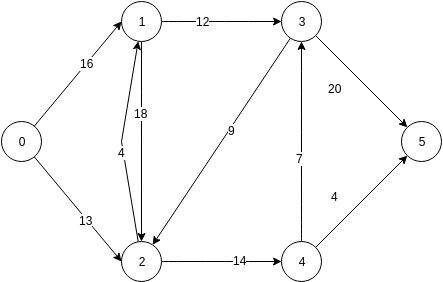
\includegraphics[width=0.8\textwidth]{flow}
	\caption{Example Flow Graph}
	\label{fig:flow}
\end{figure}


\end{document}
